\documentclass[letterpaper, 10 pt, conference]{ieeeconf}  % Comment this line out if you need a4paper
\IEEEoverridecommandlockouts
\overrideIEEEmargins                                      % Needed to meet printer requirements.

%\usepackage{graphics} % for pdf, bitmapped graphics files
%\usepackage{epsfig} % for postscript graphics files
%\usepackage{mathptmx} % assumes new font selection scheme installed
%\usepackage{times} % assumes new font selection scheme installed
%\usepackage{amsmath} % assumes amsmath package installed
%\usepackage{amssymb}  % assumes amsmath package installed
%\usepackage{amsthm}
%\usepackage[style=ieee]{biblatex}
%\addbibresource{references.bib}
%
%%\theoremstyle{definition}
%%\newtheorem{definition}{Definition}[section]

%\usepackage{amssymb}
%\usepackage{graphicx}
%\usepackage{epstopdf}
%\usepackage{amsmath}
%\usepackage{subfigure}
%\usepackage{multirow}
%\usepackage{pbox}
%\usepackage{algorithm}
%\usepackage{algpseudocode}
%\usepackage{bm}
%\usepackage{url}


%%%%%%

%\documentclass[conference]{IEEEtran}
%
\usepackage{graphicx}

\usepackage{amsmath}

\usepackage{mathrsfs}

\usepackage{array}

\DeclareMathOperator*{\argmin}{arg\,min}
\DeclareMathOperator*{\argmax}{arg\,max}
\usepackage{amssymb}
\usepackage{mathtools}
\usepackage{algorithm}
\usepackage{algorithmic}
\usepackage{varwidth}
%\usepackage[noend]{algpseudocode}
\makeatletter
\def\BState{\State\hskip-\ALG@thistlm}
\makeatother


\newcommand\NB[1]{$\spadesuit$\footnote{NB: #1}}
\newcommand\RP[1]{$\clubsuit$\footnote{RP: #1}}

\newcommand*{\Z}{\mathbb{Z}}
\newcommand*{\N}{\mathbb{N}}
% reference package for bibtex

%\usepackage{biblatex}
%\addbibresource{mybibliography.bib}

%\usepackage[
%backend=biber,
%style=numeric,
%sorting=ynt
%]{biblatex}

%\addbibresource{mybibliography.bib}


% correct bad hyphenation here
\hyphenation{op-tical net-works semi-conduc-tor}


\begin{document}
%
% paper title
% Titles are generally capitalized except for words such as a, an, and, as,
% at, but, by, for, in, nor, of, on, or, the, to and up, which are usually
% not capitalized unless they are the first or last word of the title.
% Linebreaks \\ can be used within to get better formatting as desired.
% Do not put math or special symbols in the title.
%\title{Using Hidden Markov Models to Improve Autonomous Vehicle Decision Making - Problem Formulation}
%\title{A Hidden Markov Models-based Approach for Automotive Predictive and Assistive Control}
\title{\LARGE \bf A Hidden Markov Models-based Approach for Predictive and Assistive Control in Semi-Autonomous vehicles}
\author{Rahul Peddi and Nicola Bezzo%
\thanks{Rahul Peddi and Nicola Bezzo are with the Department of Systems and Information Engineering and the Charles L. Brown Department of Electrical and Computer Engineering, University of Virginia, Charlottesville, VA 22904, USA. Email: {\tt \{rp3cy, nb6be\}@virginia.edu}}
%\thanks{$^{2}$Esen Yel is with the Department of Systems and Information Engineering, University of Virginia, Charlottesville, VA 22904, USA. Email: {\tt ey3un@virginia.edu}}
}



%\author{\IEEEauthorblockN{Rahul Peddi$^1$ and Nicola Bezzo$^{1,2}$} 
%\IEEEauthorblockA{
%\small
%$^1$Department of Systems and Information Engineering\\
%\small
%$^2$Department of Electrical and Computer Engineering\\
%\small
%University of Virginia\\
%Email: \{rp3cy, nbezzo\}@virginia.edu}}
%\hyphenation{u-sing}


\maketitle

% As a general rule, do not put math, special symbols or citations
% in the abstract
\begin{abstract}
\end{abstract}

% no keywords




% For peer review papers, you can put extra information on the cover
% page as needed:
% \ifCLASSOPTIONpeerreview
% \begin{center} \bfseries EDICS Category: 3-BBND \end{center}
% \fi
%
% For peerreview papers, this IEEEtran command inserts a page break and
% creates the second title. It will be ignored for other modes.
\IEEEpeerreviewmaketitle



\section{Introduction}
% no \IEEEPARstart

%    Over the last few years, semi-autonomous and autonomous vehicles have become increasingly popular, but they have not replaced traditional vehicles entirely just yet. This leads to a hybrid environment; one that features vehicles of all levels of autonomy. Many of these vehicles to be equipped with some form of adaptive cruise control (ACC) or advance driver assistance systems (ADAS), both of which help the driver make safe decisions while operating the vehicle. These types of systems are forms of human-robot interaction. ACC performs actions autonomously and works at the command of a human who determines a target velocity and a safe following distance. ADAS, on the contrary, acts as an information system for human drivers. These systems, however, are limited in their capabilities as they require constant monitoring from the driver and are unable to predict if the driver will enter a dangerous situation in the future. In addition, these systems can fail to guarantee safety in rapidly transitioning environments.
    
    
%    Because these dangerous situations can occur so rapidly \NB{need citation here}, there is a need to increase the ability to guarantee safety when developing new systems \NB{what do you mean with new systems?} for human drivers. This can be done by increasing the ability to predict and adapt to what will happen in the future. A simple depiction of a danger situation is shown in Fig. \ref{fig:hiway}. \NB{figure needs improvements}

\NB{I'll go back to this later...intro needs a lot of attention!}
 
\NB{In a not far future, multiple vehicles with different level of autonomy will have to coexist and operate safely. Examples of such vehicles include cars, vessels, aerial vehicles. Different level of autonomy are available 1 to 5 for cars, hobby  }    
\NB{Semi-autonomous and autonomous vehicles are finding their way in our society rapidly. Although new advancements in sensing and autonomy are increasing safety by assisting drivers with line changing warning and assisted braking, } 
\NB{here let's talk about the trolly problem and mention that we see humans as disturbance in this work! discuss about teleoperated robotics that is still big and assistive automation}
Over the last few years, semi-autonomous and autonomous vehicles have become increasingly popular, but they have not replaced traditional vehicles entirely just yet. This leads to a hybrid environment; one that features vehicles of all levels of autonomy.
    
    Many of these vehicles are equipped with some form of adaptive cruise control (ACC) or advance driver assistance systems (ADAS), both of which help the driver make safe decisions while operating the vehicle. These types of systems are forms of human-robot interaction. ACC performs actions autonomously and works at the command of a human who determines a target velocity and a safe following distance. ADAS, on the other hand, acts as an information system for human drivers. These systems, however, are limited in their capabilities as they require constant monitoring from the driver and are unable to predict if the driver will enter a dangerous situation in the future. In addition, these systems can fail to guarantee safety in rapidly transitioning environments.
    

\begin{figure}[ht]
    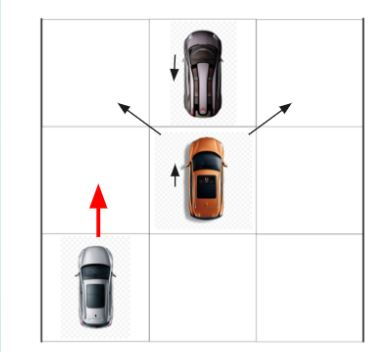
\includegraphics[width=0.5\textwidth]{highwaysit.JPG}
    \caption{A highway: a common situation in which the environment is rapidly changing. The vehicle in the center of the grid is our vehicle, and the vehicle in front is driving much slower, while the vehicle to the right is approaching very rapidly. It would be safe in the instant to pass on the left, but that leaves the possibility that a dangerous situation will occur very soon.}
    \label{fig:hiway}
\end{figure}
    
    In Fig.\ref{fig:hiway}, a  user is driving a vehicle (the vehicle in the center) in a space surrounded by other vehicles. If the driver is unaware of the future risk of performing a certain action, an unsafe situation may arise, resulting in a collision. To resolve this, we are interested in predicting future states of other vehicles, assess risk of collisions given the user's actions, and adapt the system accordingly.This type of work can be approached as a type of Markov Chain, and we leverage Hidden Markov Model (HMM) theory as well, both of which are commonly used models for many cyber-physical systems.
    
     In this work, we aim to provide
    \begin{itemize}
    \item{a prediction method that can effectively and efficiently estimate the future positions of surrounding agents}
    \item{an adaptive framework that determines the adjustment of a user's actions and severity of such adjustment that should be made at any point in time}
    \end{itemize}
  
   Although the proposed approach is applied in the context of autonomous and semi-autonomous vehicles, it is general and applicable to any other CPS. In this case, we see the user as a disturbance or an unintentionally adversarial effect. We monitor the user behavior and intervene if necessary by predicting future states of our system and the surrounding entities (obstacles and other vehicles).    
    
    The rest of this paper is organized as follows: in Section II, we discuss related work, and in Section III, we formally define the problem. The proposed AHMM framework is presented in Section IV. In Section V, we discuss a specific case study, in which our framework is applied to guarantee safety. We demonstrate our results with MATLAB simulations and real-world experiments in Sections VI and VII, respectively. Lastly, we discuss our conclusions and future work in Section VII.

    
% You must have at least 2 lines in the paragraph with the drop letter
% (should never be an issue)

\section{Related Work}

%    This work is tuned a relatively specific situation; one where the host vehicle is driving in the middle lane of a three-lane highway. This was chosen in order to account for a large action space. In this case, there are three possible actions the host vehicle could take, and each of these actions is evaluated for safety. The action space is defined such that it only looks at the immediately adjacent lanes. For example, if the vehicle is in the left lane, the action space consists of forward, and move right. In this case, only those two actions are evaluated for safety at a future time step.
    
    
%    A Hidden Markov Model is a type of Markov Model, where the states are hidden. A Markov Model examines states and transitions to and from these states. An HMM operates on the assumption that we don't directly know what the state is, but we are able to make observations that can tell us valuable information about the current state. Hidden Markov Models have been used for many human-robot interaction applications \cite{li2016modeling}, including but not limited to speech recognition, motion recognition, and biological analyses \cite{yoon2009hidden}.
    
%    In addition to the host vehicle at the center of the road, there are two additional vehicles; one passing on the left lane, and a slowed vehicle ahead in the center lane, as shown in Figure \ref{fig:actionspace}.
    
%    The HMM was performed on the blue vehicle to the left (the purple vehicle is a representation of the estimate), from the perspective of the black vehicle, the host vehicle. The testing was done such that only one vehicle was able to make estimations, but in a truly hybrid environment, multiple vehicles will this technique will improve the ability for multiple vehicles to collaborate.
    
\section{Problem Formulation}
 
In this work we are interested in finding an approach to proactively guarantee safety (i.e., something bad will never happen) in multi-vehicle systems. We focus on manned vehicles employing an hybrid autonomy scheme as defined in \cite{} in which the control authority is shared between the human and the on-board computer. For the sake of brevity we denote this class of vehicles as {\em hybrid autonomous vehicles} (HAVs), In our scheme, the on-board computer is used as a supervisory monitor to predict and assess safety and assist by correcting undesired human behaviors that may lead to unsafe situations and compromise system's integrity. 
% control in which users may perform undesired actions that can compromise the safety of the entire system 
Formally the problem that we investigate in this work can be stated as: 

\textbf{Problem 1: \textit{Proactive Safe Assisted Planning and Control}:} 
      A hybrid autonomous vehicle (HAV) $h$ is moving in an environment in the presence of other vehicles $q \in R_h(t)$, where $R_h(t)$ is a time varying set of vehicles in sensing/communication range with $h$. The goal is to find a policy to:
    \begin{enumerate}
        \item  predict online other vehicles future states $s$ and their likelihood $p$. Formally, $\forall q \in R_h(t)$:
    \begin{equation}
   S_q=\{{s_q(t), s_q(t+1),..., s_q(t+T)}\}
       \end{equation}
       \begin{equation}
   P=\{{p_q(t), p_q(t+1),..., p_q(t+T)}\}
%     \forall q \in R_h(t), S_q=\{{s_q(t), s_q(t+1),..., s_q(t+T)}\}
    \end{equation}
     where $S_q$ is the set of all states, $s_q$, and $P$ is the set of all probabilities, $p_q$ over a finite time horizon $T\in\N$.  
%     assess their likelihood
%    \begin{equation}
%    P=\{{p_q(t), p_q(t+1),..., p_q(t+T)}\}
%    \end{equation}
%    where $P$ represents the set of all probabilities, $p_q(t)$ represents the probabilities at each time, $t$.
    \item assess the risk $0\leq r \leq1$ of a collision during $T$ and
    \item assist and intervene to correct the HAV actions to guarantee safety, i.e., obtain an input policy $U_h=\{{u_h(t), u_h(t+1),..., u_h(t+T)}\}$ such that if the risk $r$ is always minimized. 
    \end{enumerate}
   In our specific multi-vehicle case, risk is a function of distance between vehicles. Hence minimizing risk is equivalent to guaranteeing the following:
    
%    surpasses a certain user defined level,$\rho$, we are able to minimize the risk, and guarantee,
    \begin{equation}
        ||{x_h(t)-x_q(t)}|| \geq d_{\textrm{min}}
    \end{equation}
     where $x_h(t)$ and $x_q(t)$ are the positions of the HAV and the $q^{\textrm{th}}$ surrounding vehicle at time $t$ and $d_{min}$ is a minimum safe distance.    
    
    It is important to note that the vehicle being modified is primarily human operated, in the sense that we should intervene only when necessary \NB{we are not modifying anything, we are adapting and assisting its operation. This sentence needs to be rewritten.}. Unless the user performs actions that we predict could lead to unsafe conditions, which we define as situations where $r_h>\rho$, with $\rho$ a user defined threshold, we let the HAV perform his/her desired actions.

\section{Approach}

In this section we propose a novel HMM-based approach to predict future states of other vehicles. We leverage a history of offline observations to build different models that are used online to recognize and predict other vehicles' behaviors. The technique derived in this work also aims to find a method to guarantee safe operation based the models. %\NB{simplify}
MPC [ref] or QMDP [ref] could be used to solve this problem as well, but in comparison to MPC and QMDP that require computationally expensive value iterations, this work is more efficient while guaranteeing safety. In this work, we train multiple models offline over a horizon $T$, with training sets that capture the behaviors of vehicles.

%\NB{In this work we train multiple models offline over an horizon {T}}

\subsection{HMM-based Training Framework} \label{sec:fmwk}

The proposed Adjusted Hidden Markov Model can be described by a tuple $\langle \mathcal{O},\mathcal{S},\mathcal{E},\mathcal{G},\mathcal{P},\mathcal{B} \rangle$  where:
\begin{itemize}
    \item $\mathcal{O}$ is a finite set of observed states $o(t)$ collected over a finite past time horizon $T$, $\mathcal{O} = \{ o(t-T), o(t-T+1), \ldots, o(t)\}$
    %\NB{change to lower t}.
    \item  $\mathcal{S}$ is set of $n$ unique values that $\mathcal{O}$ can be, pulled from a finite set $\forall o(t)\in\mathcal{O}$, $s_i \in \mathcal{S}$ denoted as $s_{i}$ or $s_{j}$, where $i,j = \{1,\ldots,n$\}, with $n \in \mathbb{N}$ and $i = \lor \neq j$. The notation $s_{ij}$ represents the state transition from $s_i$ to $s_j$.
    \item $\mathcal{C}$ is the finite set of emissions, or inferences that relate to each state, $c(t)$ collected over a finite past time horizon $T$, $\mathcal{C} = \{ c(t-T), c(t-T+1), \ldots, c(t)\}$.  
    \item $\mathcal{G}$ is a finite set of $m$ unique inferences, pulled from a the finite set $\forall c(t)\in\mathcal{C}$, $g_k \in \mathcal{G}$ denoted as $g_{k}$ where $k = \{1,\ldots,m$\}, with $m \in \mathbb{N}$
    \item $\mathcal{P}$ is a transition probability matrix with dimension $n \times n$. This matrix describes the probability of entering a certain state, $s_{j}$ at $t+1$, while currently in a particular state $s_{i}$ at $t$, defined by the equation:
        \begin{equation}
            p_{ij} = P(s_j(t+1) \vert s_i(t))
        \end{equation}
        This probability is calculated by counting the occurrences of each state transition over all transitions from that state:
        \begin{equation} \label{eq:transbuild}
            p_{ij} = N_{s_{ij}}/N_{s_{i}*}
        \end{equation}
        where $N$ represents the total occurrences of the ensuing entity, and $N_{s_{ij}} \leq N_{s_{i*}} \leq T$. The state transition matrix is right-stochastic, meaning $\sum_{j=1}^{n}(p_{ij}) = 1$ and is of the form:
        \begin{equation}
            \mathcal{P} = 
                    \begin{bmatrix}
                        p_{11} & \dots & p_{1n} \\
                        \vdots & \ddots & \\
                        p_{n1} &    & p_{nn}
                    \end{bmatrix}
        \end{equation}
    \item $\mathcal{B}$ represents the emission, matrix, which lists the probability that given a state, $s_i$ where $i = 1,\ldots,n$, we can expect a certain emission. This is defined by the equation:
        \begin{equation} \label{eq:obsref}
            b_{ik} = P(g_k(t+1) \vert s_i(t))
        \end{equation}
        where $i = \{1,\ldots,n\}$. The emission probabilities are calculated in a similar way to (\ref{eq:transbuild}):
        \begin{equation} \label{eq:obsbuild}
            b_{ik} = N_{g_{ik}}/N_{g_{i*}}
        \end{equation} 
        where $N_{g_{ik}} \leq N_{g_{i*}} \leq T$. This matrix is of the size $n\times m$:
        \begin{equation}
            \mathcal{B} = 
                    \begin{bmatrix}
                        b_{11} & \dots & b_{1m} \\
                        \vdots & \ddots & \\
                        b_{n1} &    & b_{nm}
                    \end{bmatrix}
        \end{equation}
        The matrices $\mathcal{P}$ and $\mathcal{B}$ will be referenced as ``the parameters" of the AHMM in the rest of this work. 
\end{itemize}

This framework is executed over $T$ and a set of parameters is obtained: $\langle \mathcal{P}, \mathcal{B} \rangle$, with implicit parameters $m$ and $n$. The AHMM is different from a traditional HMM because the states are not hidden, and we know exactly the relationship
%\NB{clarify}
between states and their corresponding inferences. Because we have all the states and transitions a priori, we can learn the parameters of multiple models offline. In addition, having the knowledge pertaining to the relationship between states and inferences allows predictions to be made with increased accuracy.
The general pictorial representation of the AHMM is shown in Fig.\ref{fig:hmm}. In this image, nodes labeled $s$ represent the states ($\mathcal{S}$), while those labeled $c$ represent the emissions ($\mathcal{C}$). The lines with the label $p$ represent the transition probabilities between states, and those labeled $b$ represent the probability that each of the connected observations are associated with connected states.

\begin{figure}[ht]
    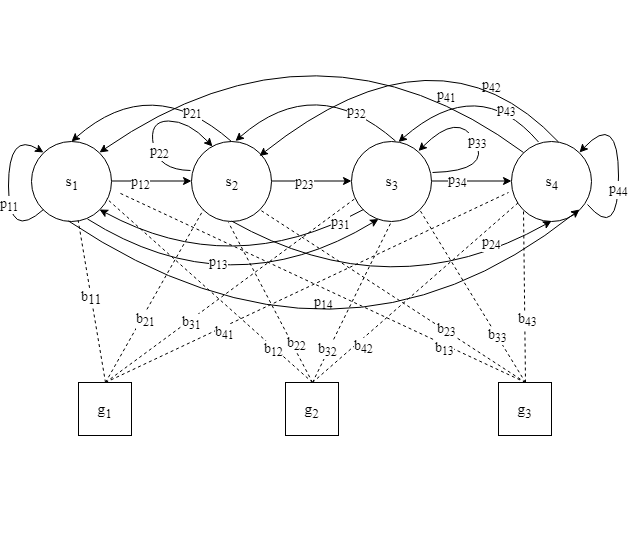
\includegraphics[width=0.5\textwidth]{ahmm.png}
    \caption{General Representation of an Adjusted Hidden Markov Model. In this image, states, emissions, and respective transition and emission probabilities are shown}
    \label{fig:hmm}
\end{figure}

The specific environment we are studying, involves three lanes with multiple vehicles that can change their velocities and their lanes. Within this environment, we are able to set up two AHMMs to capture the behaviors we expect to see. The AHMMs are applied to all of the agents, $q$ in our sensing range $R$.

The first AHMM will aim to predict future velocities of the agents. In this model,

\begin{equation}
\{s_1,\ldots s_n\} = \{v_1,\ldots v_n\}
\end{equation}
    where $v$ represents velocity. The emissions reflect the relationship between $v(t)$ and $v(t-1)$:

\begin{enumerate}
    \item Speeding Up, where $v(t) > v(t-1)$
    \item Slowing Down, where $v(t) < v(t-1)$
    \item Maintaining Speed, where $v(t) \approx v(t-1)$
\end{enumerate}

The second AHMM will be used to predict the lateral position of the agents. The positions, for our purposes, are modeled as discreet lanes: (Left, Center, Right);

\begin{equation}
    \mathbf{L} = \{L,C,R\}
\end{equation}

In this model, states represent distances between preceding agents:

\begin{equation}
\{s_1,\ldots s_n\} = \{d_1,\ldots d_n\}
\end{equation}

where $d$ represents the distance between the relevant agent, $q$, and a preceding agent its lane. The emissions reflect reactions to the preceding agent and are as follows:
\begin{enumerate}
    \item Changing Left
    \item Changing Right
    \item Not Changing
\end{enumerate}
In this case, the relationship between states and emissions indicates at what distance $d_n$ we can expect the agent to react to the preceding agent.

\subsection{AHMM-Based Online Prediction and Updating} \label{sec:ahmmpredupdate} %\NB{perhaps combine with next and add Update in the title}
 Using the framework above, we build a model of a certain system offline. At $t$, the parameters of the AHMM can be used to make online predictions about the future states of the observed system. This is done by identifying the current state, $s_{i}(t)$ and applying it to the transition and emission matrices, which are used as lookup tables, to obtain the next most likely state and its likelihood. We start with the assumption that $\mathcal{P}$ will give conclusive results from which we can predict the future state as follows:
\begin{equation} \label{eq:nextstate}
    s_{i}(t+1) = \max_{j}[\mathcal{P}_{i(t),j}]
\end{equation}
There is, however, the possibility that there will be more than one returned states, as the maximum transition probability can be the same for multiple states. In this situation, we invoke the use of $\mathcal{B}$:
\begin{equation} \label{eq:nextemis}
    g_{k}(t+1) = \max_{k}[\mathcal{B}_{i(t),k}]
\end{equation}
%\NB{equation needed}. 
Because the relationship between states and observations is not hidden, we can use the expected inference, derived from (\ref{eq:nextemis}) to assess which returned state is more accurate. In the event that the prediction is still unclear, meaning that more than one of the states returned from \ref{eq:nextstate} satisfy the expected inference, we elect the more dangerous transition, which depends on the specific application. For instance, in our case study, the more dangerous transition is one that minimizes the distance between our user's vehicle and the observed vehicle. Using this method, it is possible to predict the future states using the transition and emission matrices over any user-set horizon $H$, assuming that the prediction is correct at each iteration. %\NB{flip the order} \NB{explain the algorithm}.
The algorithm below shows how we carry forward this prediction through $H$, as shown in Algorithm \ref{alg:pred}. In this algorithm, an observed state, $s(t) = s_i$, is used with $\mathcal P$ and $\mathcal B$ to find the most likely next state, $s(t+1) = s_{j*}$. The following state, $s(t+2)$ is calculated using $s_{j*}$ as though it is an observed state. This process is repeated up to $t+H$. 

\begin{algorithm}[ht!]
\caption{Future State Prediction} \label{alg:pred}
\begin{algorithmic}[1]
\WHILE{$t\leq t+H$}
\STATE $t \gets t+1$
\FOR{$s(t) = s_i$}
\STATE $j* \gets \max_j(\mathcal{P}_{i}*)$
\ENDFOR
%\IF{$j$ is not a singleton}
%\FORALL{$j$}
%\STATE{$k \gets j-i$}
%\ELSE
\STATE $s(t+1) \gets s_{j*}$
%\ENDFOR
%\ENDIF
\ENDWHILE
\end{algorithmic}
\end{algorithm}

In addition, AHMM parameters can be updated online in order to increase the accuracy of the model. This is done by using (\ref{eq:transbuild}) and (\ref{eq:obsbuild}) the new transition and associated observation. In the aforementioned equations, $N_{s_{ij}}$ and $N_{g_{ik}}$, will change, and therefore, $p_{ij}$ and $b_{ij}$ will change. As a result, new parameters $\mathcal{P'}$ and $\mathcal{B'}$ are created to reflect the updates. In addition, we use a sliding window approach such that the size of the training set is always $(t-T)$, where $t$ is the current time, and $T$ is the time horizon of the training set. The training set is kept the same size in order to retain computational efficiency. $\mathcal{P'}$ and $\mathcal{B'}$ will continue to be used for online prediction. %\NB{rewrite}

\subsection{Online Model Fitting}\label{sec:omf} %\NB{label for sections}
Using the framework described in Sections \ref{sec:fmwk} and \ref{sec:ahmmpredupdate},  we can extract a model that captures the behavior of a system that we have been observing for $T$. Multiple models can be extracted using several data sets, and with that we can obtain super-sets containing all the transition and emission matrices: 
\begin{equation}
    \hat{\mathcal{P}} = \{\mathcal{P}_{N_{1}},\ldots,\mathcal{P}_{N_{M}}\}
\end{equation}
\begin{equation}
    \hat{\mathcal{B}} = \{\mathcal{B}_{N_{1}},\ldots,\mathcal{B}_{N_{M}}\}
\end{equation}
where $\mathcal{N} = \{N_1,\ldots,N_M\}$, where $M$ represents the number of models and $M\in\mathbb{N}$.
During run-time we observe new measurements of other vehicles and the challenge becomes fitting each new vehicle's observations to the right model. However, until we have enough data about this new system, the prediction may not be correct, and thus, we need to take into account error, $e$. In efforts to minimize situations where transitions are unclear, we propose training multiple models prior to the prediction process.

Having built multiple models, we observe a new vehicle and begin to execute the framework discussed in Section \ref{sec:fmwk} for two consecutive measurements, $\left[o(t-1),o(t)\right]$. With this information, we are able to further execute the framework and determine parameters $\tilde{\mathcal{P}}$ and $\tilde{\mathcal{B}}$, which stand for the transition and emission matrices for the system we are currently observing. In order to determine the optimal model, we calculate the set of errors, $\hat{e}_{N_{M}} = \{e_{N_1},\ldots,e_{N_M}$\} between our model and each of the offline models:

\begin{equation}
    \forall{N_M} \in \mathcal{N}: \hat{e}_{N_M} = \lVert\tilde{\mathcal{P}}-\hat{\mathcal{P}}_{N_M}\rVert_{l1/l2}
\end{equation}

In order to determine the model with the lowest error, we minimize the set $\hat{e}_{N_M}$,

\begin{equation}
    N_M^* = \argmin_{M}(\hat{e}_{N_M})
\end{equation}
%\NB{add argmin}

where $N_M^*$ represents the model with the least error, or the optimal model. In order to make predictions using the optimal model, we refer to the parameters, $\mathcal{P}_{N_M}$ and $\mathcal{B}_{N_M}$. The procedure to predict future states is shown in Algorithm \ref{alg:pred}.

%\NB{merge with previous and change to explain better how new data are going to improve your model...Bellman optimality}
If the observed system, however, does not result in an $N_M^*$ with a low error, the model is updated using the method discussed in Section \ref{sec:ahmmpredupdate}. Because we are attempting to fit the model, rather than build a new one, we have the advantage of having the baseline, the current $N_M^*$. We are able to leverage the parameters of this model, by  updating $\mathcal{P}_{N_M^*}$ and $\mathcal{B}_{N_M^*}$ as we observe new transitions or make new inferences, much like how we obtain $\mathcal{P}'$ and $\mathcal{B}'$ in Section \ref{sec:ahmmpredupdate}. In this case, we obtain $\mathcal{P}'_{N_M^*}$ and $\mathcal{B}'_{N_M^*}$. These models to make future predictions using Algorithm \ref{alg:pred}.

%\subsection{System Model}
%The vehicle we use in our case study is a human-controlled vehicle with autonomous capabilities. The model used for the vehicle is that of a unicycle-type robot:
%\begin{equation}
%    \begin{cases}
%    \dot{x} = u_s\cos{\theta} \\
%    \dot{y} = u_s\sin{\theta} \\
%    \dot{\theta} = u_\omega
%    \end{cases}
%\end{equation}
%where $(x,y,\theta)$ is the vehicle's position and orientation, and $(u_s,u_\omega)$ is the input control pair that represents linear and angular velocities. The inputs consist of autonomous and human controlled parts, $u_a$ and $u_h$. These values always satisfy the criteria $u_a+u_h = 1$. This vehicle will be known as the host vehicle, as it is where the computation takes place. In addition, all vehicles within a certain sensing range of the host vehicle are modeled as follows:
%\begin{equation} \label{eq:agentpos}
%    \forall q \in R:
%    \begin{cases}
%    \dot{x}_q = v_q\cos{\theta_q} \\
%    \dot{y}_q = v_q\sin{\theta_q} \\
%    \dot{\theta}_q = \omega
%    \end{cases}
%\end{equation}
%where $q$ represents each vehicle in sensing range $R$. In our case, however, we modify these models such that actions in the lateral direction are discreet, and there is no angular velocity. This is done because in the scope of this work, we not concerned with the trajectory of the lane change; just the fact that it is going to happen. These vehicles, $q$ will be referred to as agents in the remainder of this work.

%\subsection{Environment Setup}

%Multiple models can be trained using the AHMM framework, yielding $\mathcal{P}$ and $\mathcal{B}$ matrices for each model, and these models can be used for fitting, updating, augmentation, and most importantly, prediction, as discussed in the previous sections. Using the method for fitting models, we are able to identify $N_M^*$ from a set of pretrained models, which consists of the appropriate AHMM parameters for the optimal model, for both velocity and lateral position.

\subsection{Using AHMM Method for Safe Vehicle Operation}
In this section, we discuss how the AHMM method is used to guarantee safety for a vehicle. In this situation, we have our manned vehicle, $h$, and we have all of the vehicles in our vehicle's sensing range, $R_h$:
\begin{equation}
    \forall{q}\in R_h, q = \{1,\ldots,N_{R_h}\},
\end{equation}
where $N_{R_h}\in\mathbb{N}$ and represents the total number of vehicles in the sensing range. These vehicles will be referred to as agents in the rest of this work.

Generating and using the optimal model for each vehicle $q$, as discussed in Section \ref{sec:omf}, we are able to predict where an agent will be in the environment for the user-defined time horizon, $H$, as discussed in Section \ref{sec:ahmmpredupdate}. This time horizon defines how far ahead the user wants the system to check, in order to intervene. A sequence of future states for agent $q$, both in terms of velocity and lateral position, are developed for $H$ using the AHMM parameters and Algorithm \ref{alg:pred}. Given a sequence of future predicted velocities,
\begin{equation}
    v_q^p = \{v_q(t+1),\ldots,v_q(t+H)\}
\end{equation}
we are able to calculate the forward positions for the horizon $H$ using:
\begin{equation} \label{eq:dumpos}
    x_q(t) = v_q*\delta
\end{equation}
where $\delta$ refers to a sampling time. With this we obtain
\begin{equation}
    x_q^p = \{x_q(t+1),\ldots,x_q(t+H)\}
\end{equation}
Using this information, we build a risk profile and adapt the host vehicle's input accordingly.


\subsection{Risk Estimation based on Online Prediction}
This section shows how risk is defined given our online prediction over $H$. Generally, risk will be calculated for each possible action the driver could take. In this case, risk will be calculated as a separate entity for each lane, $l$, and $l\in\mathbf{L}$

In this case, we also assume that the driver will continue the behavior he/she is doing at $t$ up to $t+H$. With this assumption, we are able to the estimate the future positions of $h$, obtaining the set:
\begin{equation}
    x_h^p = \{x_h(t+1),\ldots,x_h(t+H)\}
\end{equation}

Risk is a function of the distance between estimated future positions of the host vehicle and those of the agents. The distance is calculated using the following equation:

\begin{equation}
    \forall q \in R \land \forall t\in H : d_q(t) = \lVert x_h(t)-x_q(t)\rVert
\end{equation}

We will use $r$ to denote this risk, which increases as distance decreases. The following equation demonstrates how we calculate risk:

\begin{equation}
\forall{t}\in H::
    r_{q}^{l}(t) =
    \begin{cases}
    1,                      & \text{if } d_{q}(t) < 1 \\
    \frac{1}{d_{q}(t)},  & \text{otherwise} 
    \end{cases}
\end{equation}

where $r_{q}^{l}(t)$ represents the risk of a certain agent $q$ interfering with the user's position in a certain lane $l$. The set of all risks for each vehicle will be denoted as $\mathcal{R}_q$, where

\begin{equation}
    \forall{q} \in R: \mathcal{R}_q =
                    \begin{bmatrix}
                        r_q^L(t+1) & \dots & r_q^R(t+1) \\
                        \vdots & \ddots & \\
                        r_q^L(t+H) &    & r_q^R(t+H)
                    \end{bmatrix}
\end{equation}

It is important to note that multiple agents affect risk in our analysis, the agent with the highest risk is considered for adaptation. The set of maximum risk values for each lane at each time is evaluated as follows:

\begin{equation}
    \forall{l}\in\mathbf{L}:\hat{r}^l =  \max_{r_{q}^{l}}(\mathcal{R})
\end{equation}

Using this, we obtain the maximum risk in each lane in horizon $H$. This is shown in the set:

\begin{equation}
    \hat{\mathcal{R}} = \{\hat{r}^{L},\hat{r}^{C},\hat{r}^{R}\}
\end{equation}

\subsection{Adaptive User Assistance}

Given the $\hat{r}$ values for each lane for all $t\in H$, we can adapt our user's potentially unsafe actions to guarantee safety. In order to adapt, we need to first identify whether these actions are going to result in a dangerous situation. A user parameter, $\rho$ is used as a threshold for risk. This value must satisfy the condition: $0<\rho<1$. A high $\rho$ would indicate that the user is willing to incur more risk, while a lower $\rho$ would indicate a more conservative driver. Given this value, our system does not interfere with the actions of the vehicle unless the maximum risk in the user's lane surpasses $\rho$, as is shown below:

\begin{equation}
    u_a > u_h \iff \hat r^{l_u} > \rho
\end{equation}

where $u_a$ and $u_h$ represent autonomous and human inputs, while $l_u$ represents the user's lane and $l_u \in \mathbf{L}$. In the case that the autonomous control input surpasses that of the user input, the system analyzes the correct action to take. Because the risk is calculated for each lane, the initial action is to identify if a certain lane has a lower risk. With this, we identify $l^*$, which is the lane with the lowest risk:

\begin{equation}
    l^* = \min_l(\mathcal{\hat{R}})
\end{equation}

In addition, we determine the minimum and maximum velocities our vehicle should be driving within one lane. These values are calculated as follows:

\begin{equation}
    v_{\min} = d_{q,\min}/\delta
\end{equation}

\begin{equation}
    v_{\max} = d_{q,\max}/\delta
\end{equation}

This is done so that there is a method for velocity control as well, in the case that a lane change is unfeasible, or more risky than maintaining $l_u$.
% Let us take, for example, our host vehicle travelling at a much higher velocity than a preceding agent in the same lane. Our system identifies that our user has not shown any sign of turning, and because of that, we assume the user's priority is to stay in the lane. As a result of this, the $u_a$ involves lowering the velocity first. Assuming that the user doesn't respond, our system will continue to lower the velocity such that $u_s = v_q$, as long as the risk remains below $\rho$. If the user responds with a sub-optimal lane change, then the system will assist the user by reverting to the optimal action instead.  


\section{Simulations}
The simulations for this work primarily were done in Matlab. Different simulations were run for each part of the approach and case study shown above. We first discuss how the models were trained, and we validate those results for both velocity and lateral positions. This is followed by showing an example of fitting one model given multiple pre-trained models and a new system to observe. Lastly we demonstrate the risk estimates, and the adjustments made to user actions, in order to verify that we are able to guarantee safety.

\subsection{Training Models}
For training the models, we used a workspace featuring $15$ stationary obstacles. A test vehicle drove through a highway setting with these obstacles, and it was observed for a training period of 700 iterations. This is followed by an estimation period of 700 iterations, which were used to validate the parameters.

\begin{figure}[ht]
    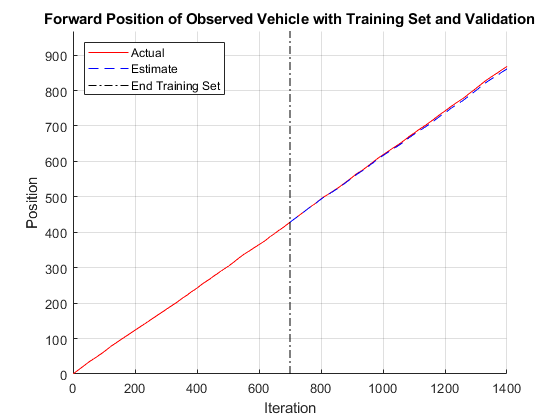
\includegraphics[width=0.5\textwidth]{train1.png}
    \caption{The forward position of the actual robot (red) is shown. After the training set, a prediction is made and the forward position of the estimate is shown (blue dashed).}
    \label{fig:train1}
\end{figure}

\begin{figure}[ht]
    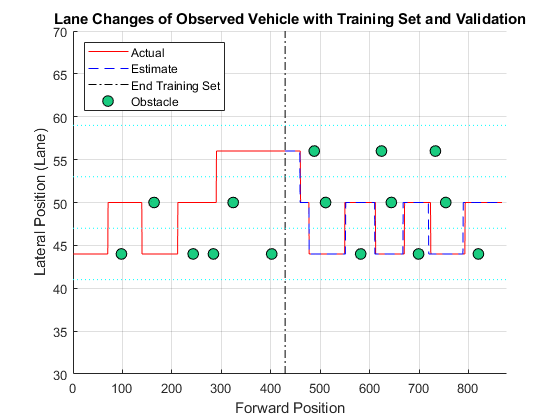
\includegraphics[width=0.5\textwidth]{train2.png}
    \caption{The lane changes of the actual robot (red) are shown. After the training set, a prediction is made and the lateral positions/lane changes of the estimate is shown (blue dashed).}
    \label{fig:train2}
\end{figure}

In this simulation we find that the root mean squared error (RMSE) between the forward positions is $3.9273$, and the RMSE between lane changes is $2.5912$.  

\subsection{Fitting Models}

In the next simulation, we show that we are able to fit pre-trained models to a certain vehicle, whose behaviors are randomly generated, moving through the same workspace as the training sets. In this simulation, we begun to fit the parameters after making one full transition and obtaining related emissions. 

\begin{figure}[ht]
    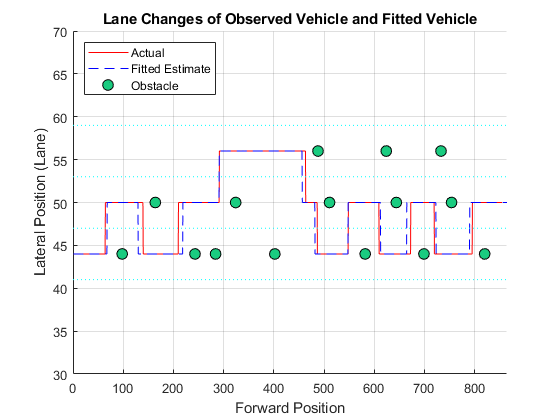
\includegraphics[width=0.5\textwidth]{fit2.png}
    \caption{The forward position of the actual robot (red) is shown. In addition, the forward position of the best-fit is shown (blue dashed).}
    \label{fig:fwd}
\end{figure}

\begin{figure}[ht]
    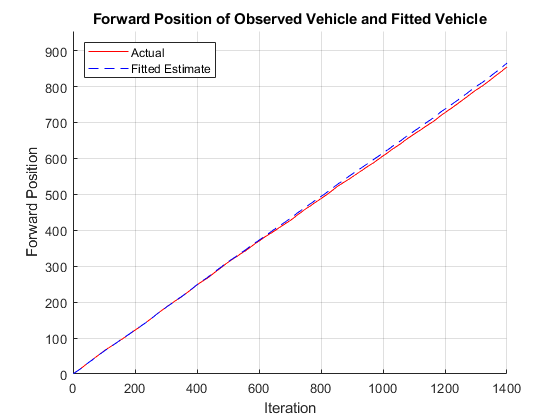
\includegraphics[width=0.5\textwidth]{fit1.png}
    \caption{The lane changes of the actual robot (red) are shown. The lane change predictions of the best-fit are shown (blue dashed).}
    \label{fig:lanchan}
\end{figure}
 In addition, we show the error of the fit for each velocity model in \ref{fig:cs1c}.
 
 \begin{figure}[ht]
    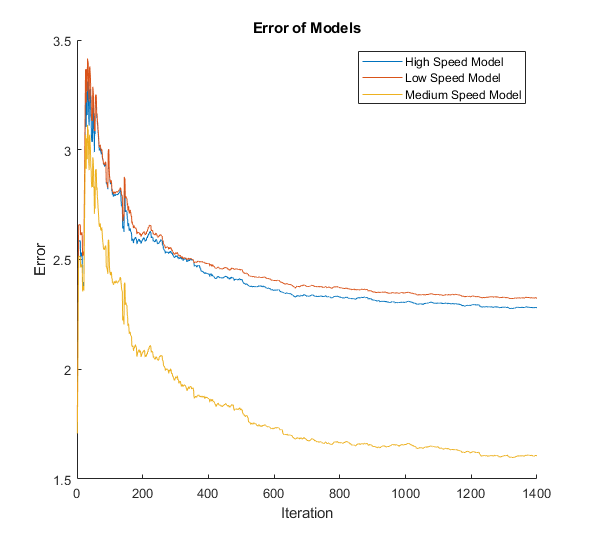
\includegraphics[width=0.5\textwidth]{fit3.png}
    \caption{The error of the fit between our model and each of the three pretrained models}
    \label{fig:error}
\end{figure}

Here we see that the closest fit is that of the medium-speed model.
 
 
\subsection{Avoidance}
In order to show the proactive safety system, we have three specific use-cases.

In the first case, the host vehicle in the center lane responds to the actions and future position of a vehicle in the left lane, which is passing a stationary obstacle. The two snapshots of the simulation in Fig.\ref{fig:cs1} and Fig.\ref{fig:cs1b} indicate the behaviors that are occurring.

\begin{figure}[ht]
    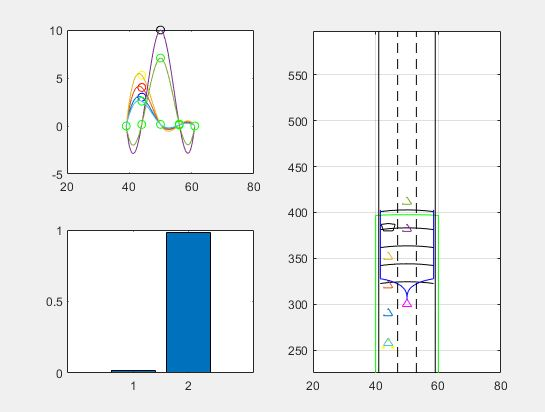
\includegraphics[width=0.5\textwidth]{cs1.JPG}
    \caption{In this snapshot, $u_{\alpha} = 0$ and $u_{h} = 1$. This is because the $r^l$ at $T_u$ is below the $\rho$.}
    \label{fig:cs1}
\end{figure}

\begin{figure}[ht]
    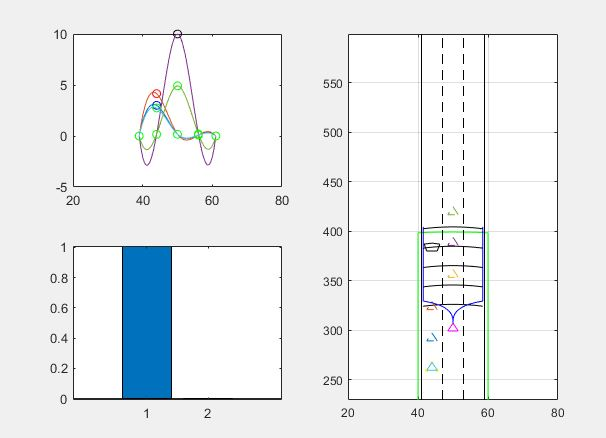
\includegraphics[width=0.5\textwidth]{cs1b.JPG}
    \caption{In this snapshot, the risk in the host vehicle's lane at $T_u$ has increased above $\rho$, and autonomy has increased rapidly. The reason $u_{alpha}$ has increased to 1, is because this is the instant at which the change begins. The location of minimum risk is determined to be the right lane, and the vehicle will then move to the right lane.}
    \label{fig:cs1b}
\end{figure}

This simulation results in a safe operation, as the minimum risk is easily identified and the solution is offered. In this simulation, the human takes no action, which is another reason fully autonomous intervention occurs, and the risk is still minimized and avoided.


In the second simulation, the human does take some action and it is evident that autonomy and human-control are fluid and change based on changing surroundings. In addition, there is once again a clear location at which the risk is at a minimum. The snapshot in Fig.\ref{fig:cs2} shows a situation where the user is travelling at a velocity slightly too rapid for the obstacle ahead, and slowing down will not put it at a risky position in relation to the next vehicle that is behind the user. As a result, $u_{\alpha}$ is increased as the level of risk increases.

\begin{figure}[ht]
    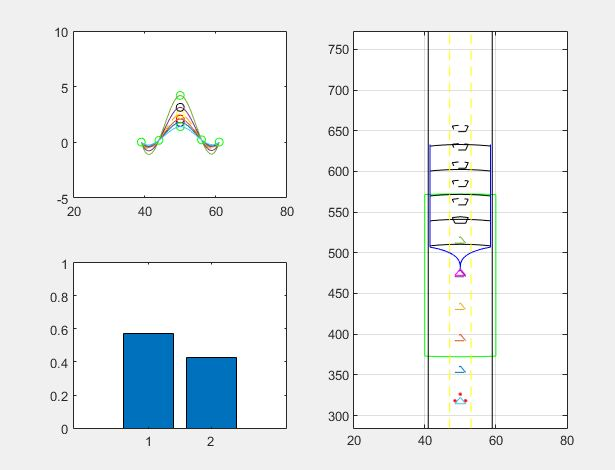
\includegraphics[width=0.5\textwidth]{cs2.JPG}
    \caption{In this snapshot, $u_{\alpha} > u_{h}$. This is because the $r^l_u$ at $T_u$ is above $\rho$}
    \label{fig:cs2}
\end{figure}

This result also indicates a case of the user's desires being met as closely as possible. The user, by only adjusting velocity and not adjusting their lane change behavior, indicates that the velocity is the first parameter to adjust. As shown in Fig.\ref{fig:cs2c}, the velocity is only adjusted so that the driver is in a safe position for the selected time $T_u$ and, consequently for times $t,t+1,\ldots,T_u$. This is indicated by a velocity that slowly decreases to a safe value. This, however, would only suffice to maximize the time before a collision occurs. Because that is a limitation of only adjusting the velocity, when a collision becomes imminent, $u_\alpha$ increases to 1, and the lane is changed to that of minimum risk.

\begin{figure}[ht]
    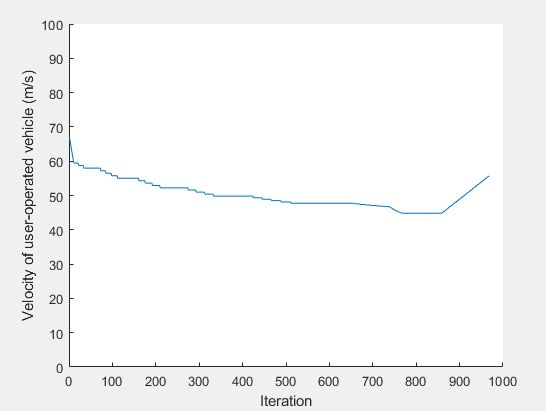
\includegraphics[width=0.5\textwidth]{cs2c.JPG}
    \caption{This figure depicts the velocity of the user's vehicle}
    \label{fig:cs2c}
\end{figure}

The third case is built much like the second case. In this implementation, however, neither of the two surrounding lanes are available. In this case, the system begins to react much like that of the second case, however, there is a error in the prediction of what the following vehicle will do. This is because the model was trained for a lane change, but it is evident that a lane change will not occur when the actual vehicle (not the estimates) approaches our user's vehicle. In a situation like this, the algorithm does delay the imminent collision, but there is a specific preference to retain a certain following distance, $d_q$ behind the obstacle in front. We assume that the user's vehicle has a responsibility to not directly cause a collision on its own. This does, however, leave the possibility of a rear collision, which is addressed further in the discussion.


\section{Experiment}
\section{Conclusions}

\newpage
% references section

% can use a bibliography generated by BibTeX as a .bbl file
% BibTeX documentation can be easily obtained at:
% http://mirror.ctan.org/biblio/bibtex/contrib/doc/
% The IEEEtran BibTeX style support page is at:
% http://www.michaelshell.org/tex/ieeetran/bibtex/
%\bibliographystyle{IEEEtran}
% argument is your BibTeX string definitions and bibliography database(s)
%\bibliography{IEEEabrv,../bib/paper}
%
% <OR> manually copy in the resultant .bbl file
% set second argument of \begin to the number of references
% (used to reserve space for the reference number labels box)

%\begin{thebibliography}{1}

%\bibitem{IEEEhowto:kopka}
%H.~Kopka and P.~W. Daly, \emph{A Guide to \LaTeX}, 3rd~ed.\hskip 1em %plus
%  0.5em minus 0.4em\relax Harlow, England: Addison-Wesley, 1999.
  
  
%\end{thebibliography}

%\printbibliography
\bibliographystyle{abbrv}
\bibliography{mybibliography.bib}


% that's all folks
\end{document}


